\chapter{Design}
\label{chap:design}

The main aim of this chapter is to design a system for the detection of the KRACK attacks in real-time. First, we propose how a testing tool for detection of a device vulnerability should work. 

\section{Testing Device Vulnerability}
\label{sec:testingTool}

Part of the assignment of the thesis was to propose a hardware or a software testing tool to detect device vulnerability to the KRACK attacks. Because the whole problem can be solved by a software tool with the necessary hardware used, we will omit possible full hardware solutions from the analysis. For testing the vulnerability, it is essential to partly or wholly perform the attack and monitor the behavior of the tested device. The principle of the attack is already described in section~\ref{sec:attackPrinciple}. Thus, we assume that the reader is now familiar with it. By tested device, we mean any wireless card in combination with the OS and the driver used. We point this out because some wireless cards might in rare cases use a different driver on the same system which might cause various behavior. We will again focus on testing the vulnerability of the 4-way handshake. Then, we will briefly discuss other handshakes.

First, we present the requirements of the tool on hardware and software. It is again necessary to have a WNIC (other than the one tested) and an OS of such combination that we can enable WNIC to be set to monitor mode. This wireless card also has to be configurable as an AP because we will run it as one. This AP simulates the rogue AP in an attacked network. Also, the AP will run our evaluating tool which should consist of a few components:

\begin{enumerate}
\item \textbf{L2 Socket}: This component can communicate on the layer 2 of the ISO/OSI model and receives data sent to a configured AP. 

\item \textbf{Parser}: This component parses data from received communication. Thus, decides which type and subtype came and what are the data in it. Its input is the received frame and the output 
are the information about the frame (e.g., it is a \textit{message~1} of the 4-way handshake containing nonce \textit{xy}, sent from the authenticator with a MAC address \textit{a} to the supplicant with a MAC address \textit{b}, etc.).

\item \textbf{Evaluator}: This component evaluates the behavior of the tested device based on the output from the parser.

\item \textbf{Logger}: This component alerts the user about results. 
\end{enumerate}

The tested device connects to our rogue AP. It does not necessarily have to forward the Internet to the client. Its main goal is to behave as an attacker and watch the answers of the client. This scenario is much easier to accomplish than the real attack because we provide the pre-shared key to the network and no MitM position is necessary to be established. The whole process of tricking the client into connection to the rogue AP, which is the hardest part, is omitted when testing device vulnerability. The AP behaves like a rogue AP regarding retransmitting \textit{message~3} of the handshake when the supplicant is in state PTK-DONE according to the state machine in Figure~\ref{fig:stateMachineSupplicant}. Based on the behavior of the client, we decide if it is vulnerable or not. To confirm the client is not vulnerable, we need to verify, that it does not reinstall the PTK (or another session key--- according to used handshake) and that it does not reset replay counter and packet number, as described in Chapter~\ref{chap:krack}.

Testing of the client side would be also similar to other handshakes. When testing the vulnerability of an AP, we would have to simulate a client which can run the evaluator component. Again, the client behaves as an attacker, and we only verify, how the victim reacts. 

\subsection{Existing Solution}

There are only a few testing tools available for testing this vulnerability. 

\subsubsection*{Official Testing Scripts}
\label{subsub:officialTestingScripts}

These scripts were published by the author of the attack and are available in~\cite{vanhoefm_2018_scripts}. They work on the principle described above meaning they simulate the rogue AP. They can be run on Kali Linux, and some users were able to run it on Ubuntu 16.04. There are a couple of prerequisites necessary to be installed prior to the execution. The scripts support a few tests each testing a different vulnerability in the 4-way, group key and Fast BSS Transition handshakes. For testing the vulnerability of the Fast BSS Transition handshake, it is necessary to have additional AP supporting 802.11r than the one tested. In these scripts, the author uses wpa\_supplicant as a rogue client and hostapd as a rogue AP. We used these scripts to test device vulnerability. The results are listed in Chapter~\ref{chap:testing} in Table~\ref{fig:tableTests}.

\subsubsection*{Wi-Fi Alliance Scripts}
These scripts are based on the scripts by Vanhoef, and their capabilities are overlapping, as described in~\cite{vanhoefm_2018_scripts}. Unfortunately, they are available only for Wi-Fi Alliance members; more information is in~\cite{wi-fi_alliance_2017}.

\subsubsection*{Tests Implemented in \textit{hostapd} and \textit{wpa\_supplicant}}
Hostapd (more information:~\cite{malinen_2013}) is a user space daemon software enabling a network interface card to act as an access point. wpa\_supplicant (more information:~\cite{malinen_2013_supplicant}) is a free software implementation of an IEEE 802.11i supplicant.
They include a number of extensions that allow special tests built to be used for testing functionality related to correct implementation of IEEE 802.11. For example, there are tests of the reinstallation of the GTK, PTK. Also, there is a test for FT Reassociation Request frame retransmission on an AP device. The documentation and source code can be found~\cite{git_index:hostapd_12AD}.

\section{Detection system}
\label{sec:detectionSystem}

In this section, we are going to design the system for detection of the KRACK attack against the 4-way handshake. We assume that the reader is now familiar with hardware and software requirements for network monitoring (as described in Chapter~\ref{chap:trafficMonitoring}) and that he knows the principle of the KRACK attack (as explained in Chapter~\ref{chap:krack}).

We set out to design a detection mechanism that will detect an attack on an independent device in the network. This means that the tool runs neither on a client nor on an AP in the network. Another possible way would be to detect the attack on an AP. This option is much easier and less prone to interference. However, this way there is a situation when we cannot verify that the attack was successful or not. Specifically, this happens in case the attacker does not forward the data frames right after the handshake. Besides, our way of solution allows us to monitor all networks on the channels we decided to monitor and also, it does not have any requirements on the operating system or memory of the AP.
This decision made a problem more complicated. First, we need a monitoring device for each channel we want to monitor, as shown by the analysis in Chapter~\ref{chap:trafficMonitoring} and was also experimentally confirmed. Besides, we monitor all the traffic going around, meaning we also see frames that for example will not be accepted by a device driver because of a wrong value of the replay counter or because of being malformed. Also, we have to distinguish different handshakes between the same two devices and different pairs of devices. The channels work completely separate in different processes. It was experimentally examined how many messages we can see in side channels (with wireless network card Alfa AWUS036NHA). It was found, we are not able to see the whole 4-way handshake, in most cases, we have seen only two messages. That is why we neglect these extra messages we could eventually see twice (on different channels).

In Figure~\ref{fig:design} on the left, we can see the detection system with three plugged interfaces on channels 1, 6 and 11. This picture serves for the better understanding of the designed solution. On the right, we can see a hypothetical attacker attacking a client connected to Wi-Fi router on channel 1 (only for illustrating of the design).

\begin{figure}[h!]
  \centering
  \includegraphics[scale=0.4]{img/design.png}
  \caption[Design of the detection system]{Design of the detection system.}
  \label{fig:design}
\end{figure}

There is a process running on each channel. The process must be able to:

\begin{itemize}
    \item Control the channel interface (set it up, set it to monitor mode, change the channel, etc.).
    \item Listen on the interface and monitor data.
    \item Parse the received data and evaluate as an event (i.e., received frame is a \textit{message 1} of the handshake, etc.).
    \item Evaluate events that happened in sequence according to non-malicious behavior of the 4-way handshake detect the KRACK attacks.
    \item Log events and save traffic to \texttt{.pcap} file for later examination. 
\end{itemize}

These functions correspond to the components we proposed for the testing tool in Section~\ref{sec:testingTool}. Thus, we will not list them again. We can see the relationship of these components in Figure~\ref{fig:process}.

\begin{figure}[h!]
  \centering
  \includegraphics[scale=0.4]{img/process.png}
  \caption[Relationship of components in the process]{Relationship of components in the process.}
  \label{fig:process}
\end{figure}

\subsubsection*{State Machine for Detection}
To evaluate the traffic and detect the KRACK attacks, we created a state machine of the 4-way handshake between a client and an AP. This handshake is identified by MAC addresses of both (the client and the AP) and by unique nonces (ANonce, SNonce) the AP and the client generate before sending \textit{message~1} and \textit{message~2} respectively. In Chapter~\ref{chap:trafficMonitoring}, we found characteristics that we are now going to use for this purpose. In Figure~\ref{fig:stateMachineAttack}, there is shown the final automata with only the scenarios that are relevant to detection of the KRACK attacks.

\begin{figure}[h!]
\begin{center}
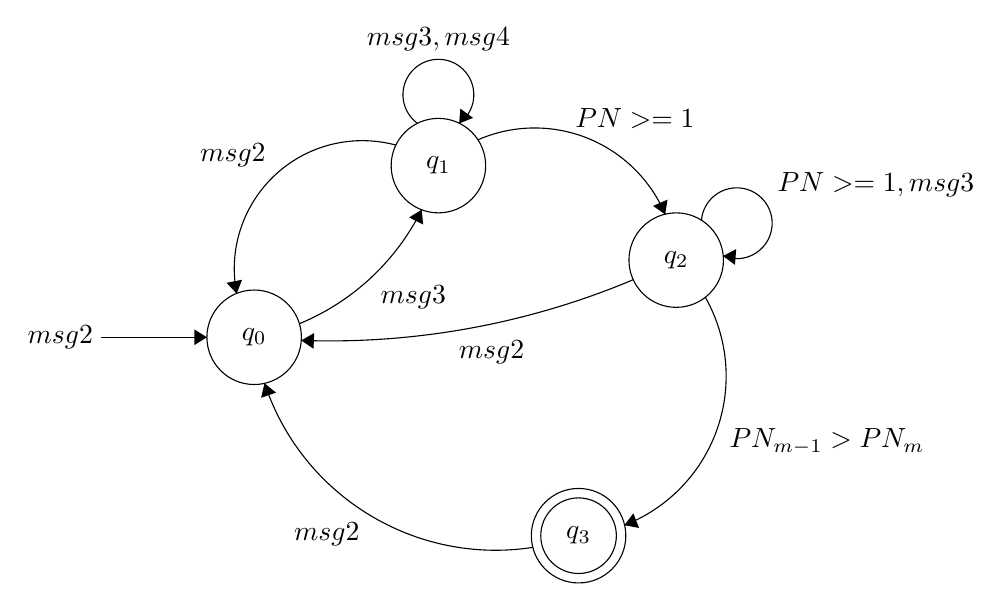
\begin{tikzpicture}[scale=0.2]
\tikzstyle{every node}+=[inner sep=0pt]
\draw [black] (22.6,-22.1) circle (3);
\draw (22.6,-22.1) node {$q_0$};
\draw [black] (34.3,-11.2) circle (3);
\draw (34.3,-11.2) node {$q_1$};
\draw [black] (49.4,-17.2) circle (3);
\draw (49.4,-17.2) node {$q_2$};
\draw [black] (43.2,-34.7) circle (3);
\draw (43.2,-34.7) node {$q_3$};
\draw [black] (43.2,-34.7) circle (2.4);
\draw [black] (12.9,-22.1) -- (19.6,-22.1);
\draw (12.4,-22.1) node [left] {$msg2$};
\fill [black] (19.6,-22.1) -- (18.8,-21.6) -- (18.8,-22.6);
\draw [black] (36.799,-9.565) arc (113.64657:23.01253:9.009);
\fill [black] (48.7,-14.3) -- (48.85,-13.36) -- (47.93,-13.76);
\draw (46.78,-8.89) node [above] {$PN>=1$};
\draw [black] (21.494,-19.33) arc (-168.7936:-285.26104:8.135);
\fill [black] (21.49,-19.33) -- (21.83,-18.45) -- (20.85,-18.64);
\draw (21.25,-11.31) node [above] {$msg2$};
\draw [black] (33.239,-14.001) arc (-26.43088:-67.62377:15.095);
\fill [black] (33.24,-14) -- (32.44,-14.49) -- (33.33,-14.94);
\draw (32.7,-18.81) node [below] {$msg3$};
\draw [black] (32.977,-8.52) arc (234:-54:2.25);
\draw (34.3,-3.95) node [above] {$msg3, msg4$};
\fill [black] (35.62,-8.52) -- (36.5,-8.17) -- (35.69,-7.58);
\draw [black] (51.001,-14.677) arc (175.32869:-112.67131:2.25);
\draw (55.8,-12.42) node [right] {$PN>=1, msg3$};
\fill [black] (52.38,-16.94) -- (53.13,-17.5) -- (53.21,-16.5);
\draw [black] (51.244,-19.552) arc (29.63405:-68.65106:10.156);
\fill [black] (46.11,-34.03) -- (47.04,-34.21) -- (46.68,-33.28);
\draw (52.75,-28.73) node [right] {$PN_{m-1}>PN_m$};
\draw [black] (46.671,-18.445) arc (-67.19541:-92.08203:49.722);
\fill [black] (25.59,-22.3) -- (26.37,-22.83) -- (26.41,-21.83);
\draw (37.67,-22.27) node [below] {$msg2$};
\draw [black] (40.298,-35.442) arc (-81.20921:-161.69491:15.457);
\fill [black] (23.26,-25.02) -- (23.04,-25.94) -- (23.99,-25.62);
\draw (27.21,-33.85) node [below] {$msg2$};
\end{tikzpicture}
\end{center}
\caption[State machine of the 4-way handshake with acceptance state of the KRACK attack]{State machine of the 4-way handshake with acceptance state of the KRACK attack.}
 \label{fig:stateMachineAttack}
\end{figure}

We receive many different types of frames but except the EAPOL frames and encrypted data frames, we ignore them. When we get in a specific state of the machine a different input than we expected (that is not listed next to transitions), we ignore it and stay in the same state. The initial state of the machine is the state $q_0$. We transition there when we receive \textit{message~2} and we store a value of the SNonce used in this message. When we get \textit{message~3}, we transition to the state $q_1$. We store the ANonce used in this message and now, we uniquely identified the handshake. We are waiting for encrypted data frames in $q_1$. When we get them, we are looking at the packet number received. It can and it will be reset after the handshake is finished, but we have to store the information about it to recognize when it happened for the second time. We look at two scenarios with one uniquely identified handshake. First, we detect the packet number is reset twice. Second, we missed the encrypted data frame with the reset packet number but we got another data frame and its packet number is lower than the one we have seen before. These two scenarios are listed in states $q_1$, $q_2$, $q_3$. In the acceptance state $q_3$, the KRACK attack is detected.



